\section{Oscilloscope GUI}
    Our oscilloscope graphical interface has been built using the QT framework for C++. Qt is a cross-platform application development framework for creating graphical user interfaces. \cite{qt-w} 
    We chose Qt as we believe that it is the most documented and practical library for GUI development in C++, using Qt allows us to create usable interfaces quickly, while being able to easily pair the backend code of C++ to the frontend.

    The interface is composed of a main window, where widgets can be attached to it easily. Everything that can be seen is customisable widgets. This allows for easy reusability, modification and removal without great refactoring due in other parts of the system.
\iffalse
    In the photo below we can see each top level widget (a QWidget that contains other widgets) in the main window, the widgets could easily be switched to other places of the window or rearranged.
    \begin{figure}[H]
        \begin{center}
            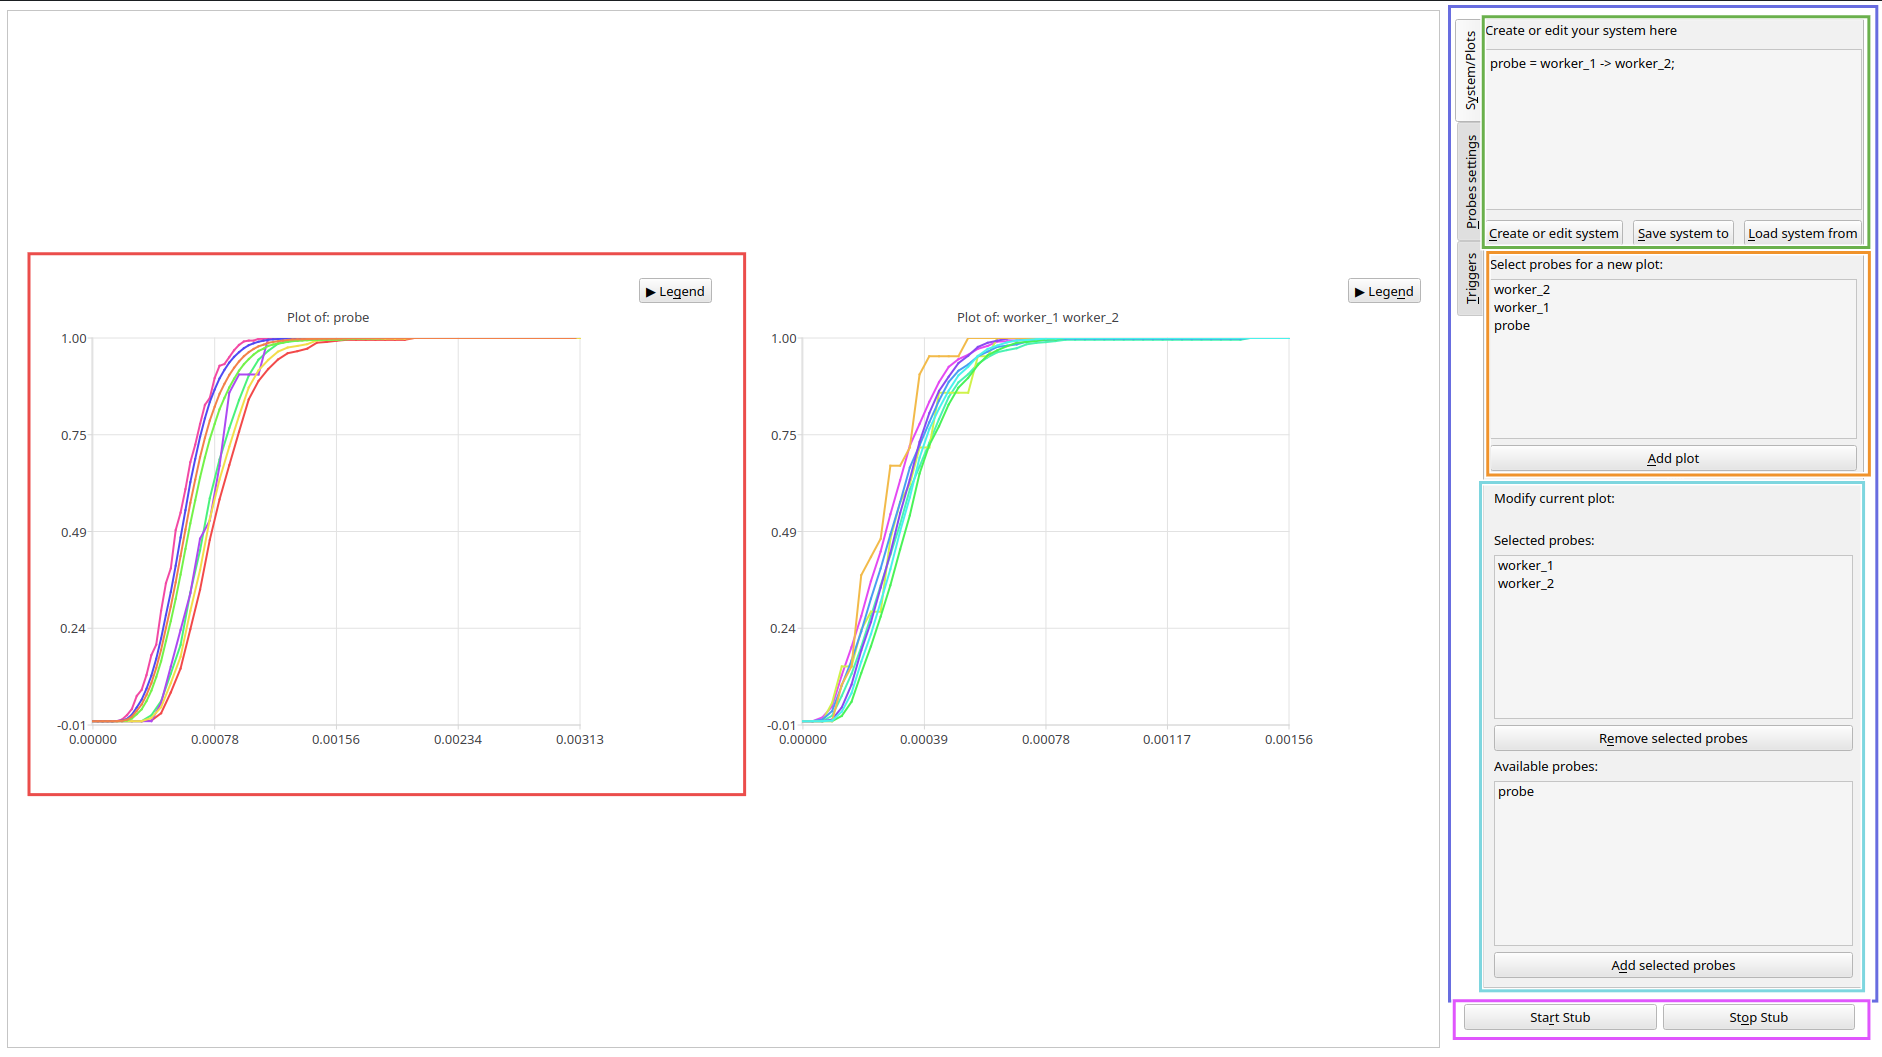
\includegraphics[width=\textwidth]{img/osc_an.png}
        \end{center}
        \caption{The oscilloscope displaying probes, the boxes represent a top level widget, which may contain other widgets inside.}
    \end{figure}

\fi
